\begin{task}{445}
Постройте \textbf{троичную} последовательность де Брёйна порядка три, начинающуюся с «\(012010\ldots\)». Сделайте это, найдя эйлеров цикл в соответствующем графе. Рисунок использованного для построения последовательности графа обязательно добавьте в решение, пронумеровав рёбра графа в порядке прохождения по эйлеровому циклу. Длина последовательности должна быть равна \(q^n+n-1\), где \(q\)~--- размер алфавита, а \(n\)~--- порядок последовательности.
\end{task}

\begin{figure}[H]
    \centering
    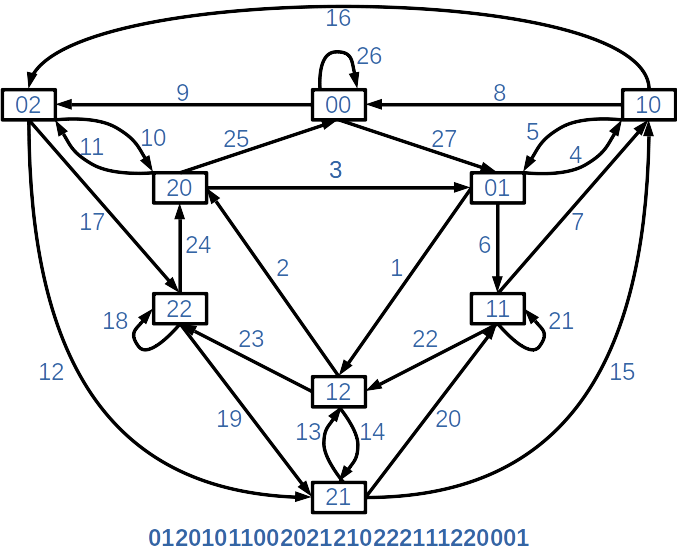
\includegraphics[scale=0.6]{Fall/img/solution-445_answer.png}
    \caption{Граф к задаче 445.} \label{graph 381}
\end{figure}

\textbf{Ответ:} 01201011002021210222111220001.
